% !TeX program = pdflatex
% Based on Elsevier's official elsarticle numbered-reference template.
\documentclass[preprint,12pt]{elsarticle}
\usepackage[T1]{fontenc}
\usepackage[utf8]{inputenc}
\usepackage{amsmath,amssymb}
\usepackage{graphicx}
\usepackage{booktabs}
\makeatletter
\let\inputtablerows\@@input
\makeatother
\usepackage{tikz}
\usetikzlibrary{arrows.meta,patterns}
\definecolor{methodInk}{HTML}{482E24}
\definecolor{methodAccent}{HTML}{A15A39}
\definecolor{methodRule}{HTML}{B99378}
\definecolor{methodPeach}{HTML}{FBE7DA}
\definecolor{methodCream}{HTML}{FFF3D8}
\usepackage{microtype}
\usepackage{enumitem}
\usepackage{needspace}
\usepackage{placeins}
\usepackage[hyphens]{url}
\newcommand{\urlprefix}{URL\enspace}
\usepackage[hidelinks]{hyperref}
\biboptions{numbers,sort&compress}
\widowpenalty=10000
\clubpenalty=10000
\journal{Journal to be selected}
\begin{document}
\begin{frontmatter}
\title{GeoEvidence-RAG: Local Geometric Evidence for Reliable Engineering Drawing Question Answering}
\author{Author names to be supplied}
\affiliation{organization={Affiliation to be supplied}}
\begin{abstract}
Engineering drawing question answering requires evidence that supports precise geometric reasoning rather than mere query similarity. Existing methods ignore local structural differences in engineering drawings; moreover, unreliable spatial reasoning under strict projection rules and geometric constraints makes decisive clues easy to overlook, often leading to incorrect answers. To bridge this gap, we propose Geometric Evidence (GeoEvidence-RAG), an evidence-oriented Retrieval-Augmented Generation framework for engineering drawings and associated CAD records. First, we propose the Local Geometric Evidence Unit, which links component and feature identities with available CAD faces, multi-view regions, geometric attributes, and provenance metadata. Second, to tackle hard negative samples in CAD drawings, we design a two-stage retrieval strategy that integrates global CLIP-based candidate selection with a lightweight evidence-aware reranking module. Furthermore, a budgeted selector is introduced to penalize redundancy while prioritizing edge-condition coverage, performing structured aggregation and explicit completeness checks across the whole corpus for given queries. Finally, we construct CADVQA, a mechanical drawing understanding benchmark comprising 3.3k high-density engineering images and 21k question-answering pairs across 9 distinct fine-grained tasks, offering a comprehensive evaluation platform to advance MLLM comprehension of real-world mechanical drawings. Extensive experimental results demonstrate that GeoEvidence-RAG achieves state-of-the-art performance across four benchmark datasets.
\end{abstract}
\begin{keyword}
Engineering Drawing Understanding \sep Retrieval Augmented Generation \sep Local geometric evidence \sep Evidence reranking
\end{keyword}
\end{frontmatter}

\section{Introduction}
\label{sec:introduction}

Mechanical engineering drawings are a primary medium for communicating geometry, tolerances, and assembly intent in mechanical design and inspection. They provide a shared technical basis for specifying component requirements, coordinating manufacturing operations, and assessing whether produced parts satisfy the intended form, fit, and function. Geometric dimensioning and tolerancing formalizes this communication through symbols and interpretation rules that relate design requirements to the features being controlled~\cite{asme2018y145}. Unlike natural images, engineering drawings encode engineering semantics through a compact, standardized graphical language that combines multiple orthographic projections, dense dimension annotations, sectional views, engineering symbols, and structured text~\cite{kou2026mechvqa}. The meaning of an individual element depends on its association with surrounding geometry and with other representations of the same component. A dimension acquires its engineering significance through the feature to which it applies, while a sectional view exposes information that may be hidden in an exterior projection. Standards governing views, sections, and cuts establish conventions for expressing these relationships consistently~\cite{iso2022views}. Accordingly, drawing comprehension involves recognizing dimensions and symbols, associating observations across views under projection constraints, and interpreting specifications using domain conventions. This dependence on spatial organization is consistent with findings in document understanding, where page layout and the relationships between textual and visual elements contribute to information extraction and question answering~\cite{xu2019layoutlm,mathew2020docvqa}. For mechanical drawings, these relationships additionally determine physical interpretations, including whether a hole terminates inside a part or whether two views depict one feature. Natural-language question answering offers a way to access this information when checking a drawing, reviewing component specifications, or comparing records in an engineering archive. Reliable answers require the relevant numerical values and graphical observations to remain connected to their features and sources, making the preservation of local engineering semantics central to drawing-based knowledge access.

Consider a drawing query that asks how many through-holes a flange contains. A search for the part name and hole diameter may retrieve the correct sheet, yet the diameter alone says nothing about where a bore ends. The answer requires matching each opening in the end view to its axial section, checking whether the bore reaches the opposite face, and counting each physical hole once. The scope of the evidence changes when the question concerns a collection of parts~\cite{li2025mechrag}. For example, even an exact volume for every retrieved part cannot establish which part is largest if the search omitted an eligible part. In both cases, the system must identify the observations needed to justify an answer and determine whether the available records supply them.

For the flange, a second end view may corroborate the location of a hole while leaving its depth unresolved. A section can settle the question only if its cutting plane passes through that same hole. For the volume comparison, the corresponding check is whether a volume is available for every eligible part and whether the values use comparable units. Figure~\ref{fig:geoevidence-workflow} shows how GeoEvidence-RAG links observations to individual features and checks the scope of a collection when the answer depends on all its members.

\begin{figure}[!ht]
  \centering
  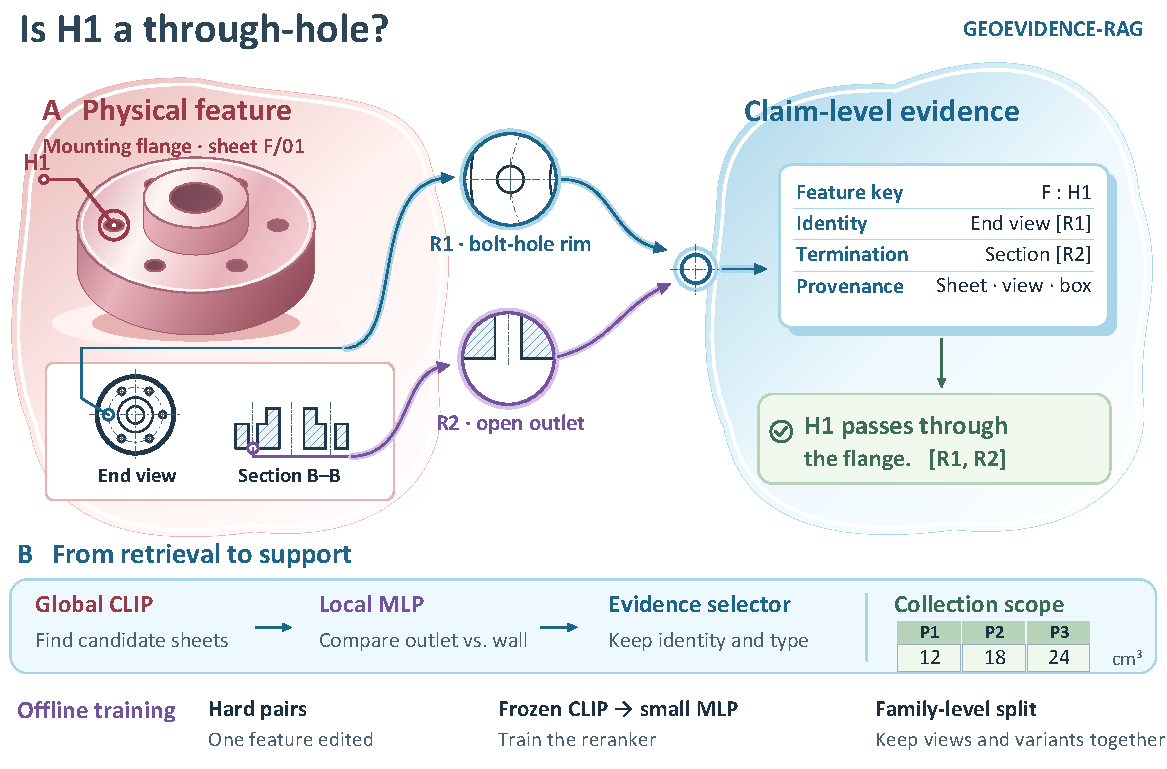
\includegraphics[width=\linewidth]{figures/workflow-plate.pdf}
  \caption{GeoEvidence-RAG illustrated on a mounting flange. (A) The end view locates bolt hole H1, and the enlarged outlet in section B--B establishes its termination. Both regions enter one feature record. A separate registry defines the population for collection queries. (B) Global retrieval supplies candidates, the local reranker compares geometry, and the selector retains the observations needed to cite the answer. The bottom strip shows how the reranker is trained.}
  \label{fig:geoevidence-workflow}
\end{figure}

The examples in Figure~\ref{fig:geoevidence-comparison} show how the value of an additional observation depends on the question. In Steps~1 and~2, the same sectional view serves two purposes. Its open exit distinguishes the through bore from a visually similar blind bore. Once the section is matched to the opening in the end view, it also confirms that the two regions describe a single feature. A second crop of the opening would repeat evidence already available, whereas the axial section supplies the missing observation about termination.

A collection query requires a different check. The largest volume in a shortlist establishes a lower bound on the collection maximum. To identify the part that attains that maximum, the system must also account for the eligible parts outside the shortlist. If a volume is missing, the system can still identify the largest part among those with known volumes and state that narrower scope.

\enlargethispage{\baselineskip}
\begin{figure}[!ht]
  \centering
  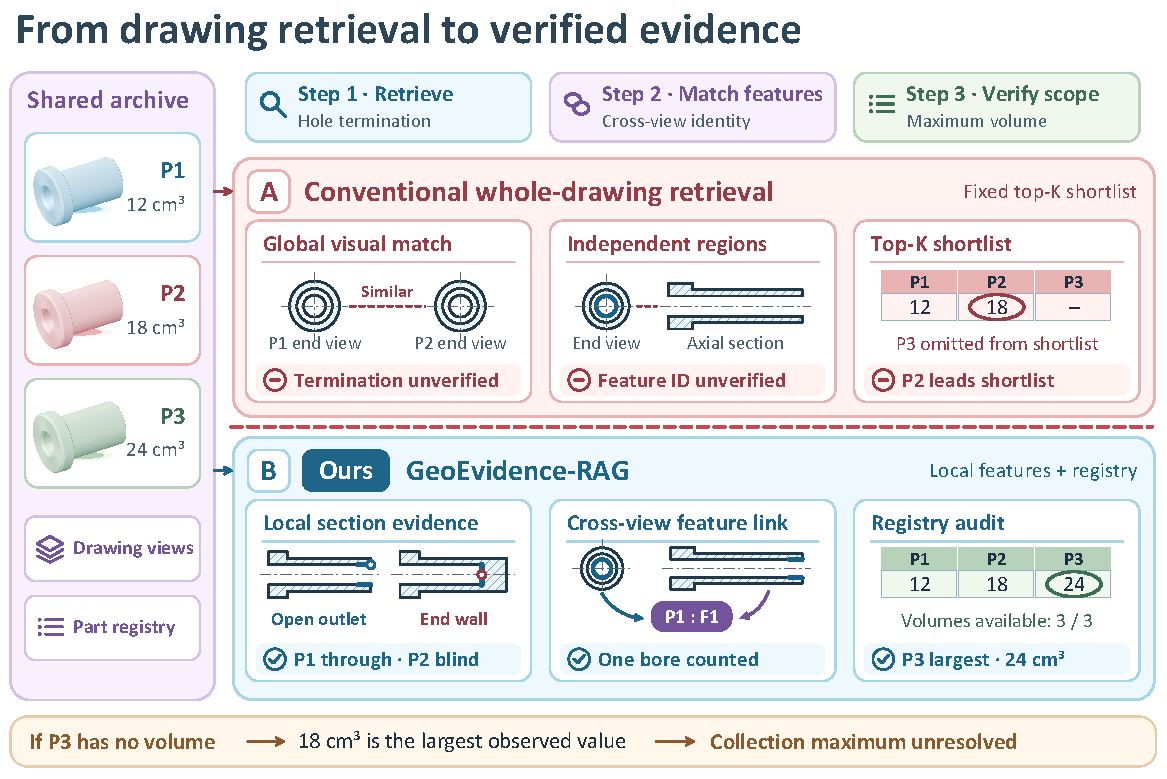
\includegraphics[width=\linewidth]{figures/counterexample-plate.pdf}
  \caption{Comparison on a shared drawing archive. (A) Conventional whole-drawing top-$K$ retrieval supplies similar end views and independent regions, and its shortlist omits P3. (B) GeoEvidence-RAG retrieves axial sections that distinguish P1's outlet from P2's end wall (Step~1), links two views of the same bore to one feature key (Step~2), and verifies that P3 has the largest volume across all eligible parts (Step~3). If P3's volume is missing, the collection maximum remains unresolved.}
  \label{fig:geoevidence-comparison}
\end{figure}

These cases expose three limitations of relying on retrieval relevance for engineering answers.

\textbf{Limitation~1: Insufficient claim-level evidence support.}\par\nopagebreak
Retrieving a relevant drawing does not establish support for each geometric claim~\cite{gao2023alce,gao2022rarr}. Reliable answers require links to the specific features, views, and attributes that justify them, such as the sectional evidence distinguishing a blind hole from a through-hole.

\textbf{Limitation~2: Limited discrimination of local geometry and cross-view identity.}\par\nopagebreak
Global semantic similarity does not guarantee correct relational interpretation~\cite{thrush2022winoground}. Parts with similar outlines may differ in hole count, termination, or coaxiality. Without explicit cross-view correspondence, repeated depictions of one feature may also be counted as separate instances.

\textbf{Limitation~3: Incomplete condition coverage and collection scope.}\par\nopagebreak
A fixed top-$K$ context may repeat observations while omitting conditions needed to answer the question. Context diversification or hierarchical organization~\cite{carbonell1998mmr,sarthi2024raptor,edge2024graphrag} does not by itself establish collection completeness. For example, the largest-volume part cannot be identified reliably if eligible parts are absent from the comparison.

To address these limitations, we propose \textit{GeoEvidence-RAG}, a framework that organizes retrieval and answer construction around verifiable local geometric evidence.
First, we construct local geometric evidence units that link part and feature identifiers to view regions, geometric attributes, and source references. We retain CAD face identifiers when available and use a shared feature identity to connect observations across views and avoid duplicate counts. We keep conflicting observations separate so that later checks can expose inconsistencies.
Then, we retrieve candidate drawings with a frozen CLIP encoder and use a lightweight multilayer perceptron to rerank them based on local geometry. We train the reranker on visually similar parts that differ in key features, including single-feature variants when editable CAD models are available. We split the data by part family, keeping original parts, their variants, and rendered views together to evaluate generalization to unseen families.
Next, we decompose each question into verifiable conditions and select complementary evidence within a fixed budget, balancing coverage, redundancy, and cost. We track which records support conditions such as feature identity, count, and termination, and flag any condition for which support is missing. For questions about totals or extrema, we check that every eligible part has the required attributes before reporting a result for the full collection. We cite the supporting records and qualify claims when evidence is incomplete.
Finally, we use our self-built CADVQA benchmark to evaluate recognition, text and table interpretation, structural reasoning, and assembly relationships. We also examine whether answers can be traced to their supporting observations.

\Needspace{5\baselineskip}
The main contributions are as follows:
\begin{itemize}[leftmargin=*,itemsep=0.45em]
\item \textbf{Local geometric evidence representation.}
We link feature and part identities to local view regions, geometric attributes, available CAD faces, and provenance, supporting cross-view consolidation and traceability from answer claims to source observations.
\item \textbf{Geometry-sensitive evidence reranking.}
We combine global candidate retrieval with a lightweight reranker designed to distinguish critical local differences, using structural hard negatives and a variant-family-disjoint training protocol with a frozen visual encoder.
\item \textbf{Complementary evidence selection with completeness checks.}
We select evidence through condition coverage, redundancy, and cost, and separately verify the collection scope and required attributes for exhaustive comparisons and aggregates.
\item \textbf{A self-built engineering drawing dataset.}
We curate drawing-based tasks spanning entity recognition, text and table interpretation, structural reasoning, and assembly relationships, providing an application-oriented setting for evaluating answers and inspecting their supporting evidence.
\end{itemize}

\section{Related work}
\label{sec:related_work}

\subsection{Document understanding and geometric representations}
\label{sec:related_understanding}

Document understanding has progressively expanded from recognizing text to modeling the relationships between textual, visual, and spatial information. LayoutLM jointly represents text and page layout and incorporates visual features associated with words~\cite{xu2019layoutlm}. LayoutLMv3 uses unified text and image masking together with word--patch alignment to support both text-centric and image-centric document tasks~\cite{huang2022layoutlmv3}. Donut follows an OCR-free approach, directly mapping document images to structured outputs and reducing dependence on a separate text-recognition pipeline~\cite{kim2021donut}. DocVQA evaluates question answering over document images and identifies document structure as an important source of difficulty~\cite{mathew2020docvqa}. These methods establish that reading words alone is insufficient for visually structured documents. Mechanical drawings introduce an additional requirement: graphical marks encode projected geometry, and observations across views may refer to one underlying feature. MechVQA addresses this domain through recognition, reasoning, and judgment tasks, together with domain-specific model training~\cite{kou2026mechvqa}. At the native CAD level, BRepNet performs message passing over boundary-representation entities, while UV-Net combines parametric surface and curve information with an adjacency graph~\cite{lambourne2021brepnet,jayaraman2020uvnet}. Their representations make geometric connectivity explicit, although their objectives differ from retrieving evidence for natural-language answers.

GeoEvidence-RAG connects these representational perspectives through a local evidence unit. A unit retains both a visible observation and the identity of the engineering feature it describes, together with attributed properties and source information. This organization lets a sectional region and an orthographic region support different conditions concerning the same feature. It also keeps the identity needed for counting separate from the number of retrieved images.

\subsection{Retrieval-augmented generation for visual and engineering documents}
\label{sec:related_retrieval}

Text-based RAG retrieves external passages and conditions generation on their contents~\cite{lewis2020rag}. Dense passage retrieval learns separate question and passage encoders, while ColBERT retains token-level interactions for fine-grained relevance scoring~\cite{karpukhin2020dpr,khattab2020colbert}. These strategies offer efficient access to large text collections, but their application to drawings depends on how graphical information is represented before indexing. A textual description can encode geometric relationships when they are explicitly extracted; ordinary OCR output or linearized text does not necessarily preserve them. Visual retrieval addresses this representational loss. CLIP learns transferable image--text alignment through contrastive supervision~\cite{radford2021clip}. ColPali represents document pages using multiple visual embeddings and matches query tokens to image patches through late interaction~\cite{faysse2024colpali}. VisRAG uses document images for both retrieval and generation, while PixelRAG retrieves web screenshots and supplies them directly to a vision-language model~\cite{yu2024visrag,wang2026pixelrag}. In mechanical engineering, MechRAG makes heterogeneous engineering records accessible through a multimodal retrieval and generation workflow~\cite{li2025mechrag}. These approaches establish useful mechanisms for preserving visual content and retrieving relevant records; their retrieval units and matching objectives provide different levels of access to local evidence.

We use a frozen visual encoder for global retrieval and a lightweight reranker to assess feature alignment, key attributes, and supporting views. We train the reranker on pairs whose geometric differences affect the answer. For editable CAD models, we modify one feature and regenerate its renderings and evidence records. To prevent data leakage, we keep each part family, including its variants and views, in the same data partition.

\subsection{Evidence attribution, selection, and collection-level reasoning}
\label{sec:related_evidence}

Several research directions improve the reliability and organization of retrieved context. RocketQA uses denoised hard negatives and data augmentation to strengthen dense retrieval~\cite{qu2020rocketqa}. Self-RAG learns to retrieve and critique evidence using reflection tokens, while corrective RAG evaluates retrieved material and can trigger corrective retrieval actions~\cite{asai2023selfrag,yan2024crag}. ALCE evaluates generated answers along dimensions including correctness and citation quality, and RARR retrieves supporting information to revise unsupported output~\cite{gao2023alce,gao2022rarr}. These studies make evidence support an explicit concern beyond fluent generation. Context selection also benefits from controlling redundancy: maximal marginal relevance balances query relevance against similarity to already selected content~\cite{carbonell1998mmr}. For broader context, RAPTOR recursively clusters and summarizes text into a retrieval tree, while GraphRAG constructs entity graphs and community summaries for collection-level questions~\cite{sarthi2024raptor,edge2024graphrag}. Their contributions address different needs, including relevance, attribution, diversity, and global synthesis. None of these objectives, considered alone, establishes that every eligible record has been included in an exact numerical comparison.

MMR balances query relevance and novelty. We decompose each question into verifiable conditions and greedily select evidence under a budget. We rank candidates by additional condition coverage per unit cost, discounting redundant observations using feature identity. This lets distinct views of the same feature contribute evidence for different conditions. We link each condition to its supporting records and flag unresolved conditions. RAPTOR and GraphRAG synthesize broader context through hierarchical and graph-based summaries, respectively. For exact numerical queries, we scan a separate registry of eligible parts and check each for a usable attribute value. We trace aggregates to their source records and limit conclusions to the observed parts when registry coverage or attribute values are incomplete.

\section{Methods}
\label{sec:methods}
GeoEvidence-RAG answers a drawing question by constructing a set of citable records. The question determines both the observations needed for a local judgment and the population needed for a collection claim. Figure~\ref{fig:method-map} places these decisions within the study.

\begin{figure}[!ht]
\centering
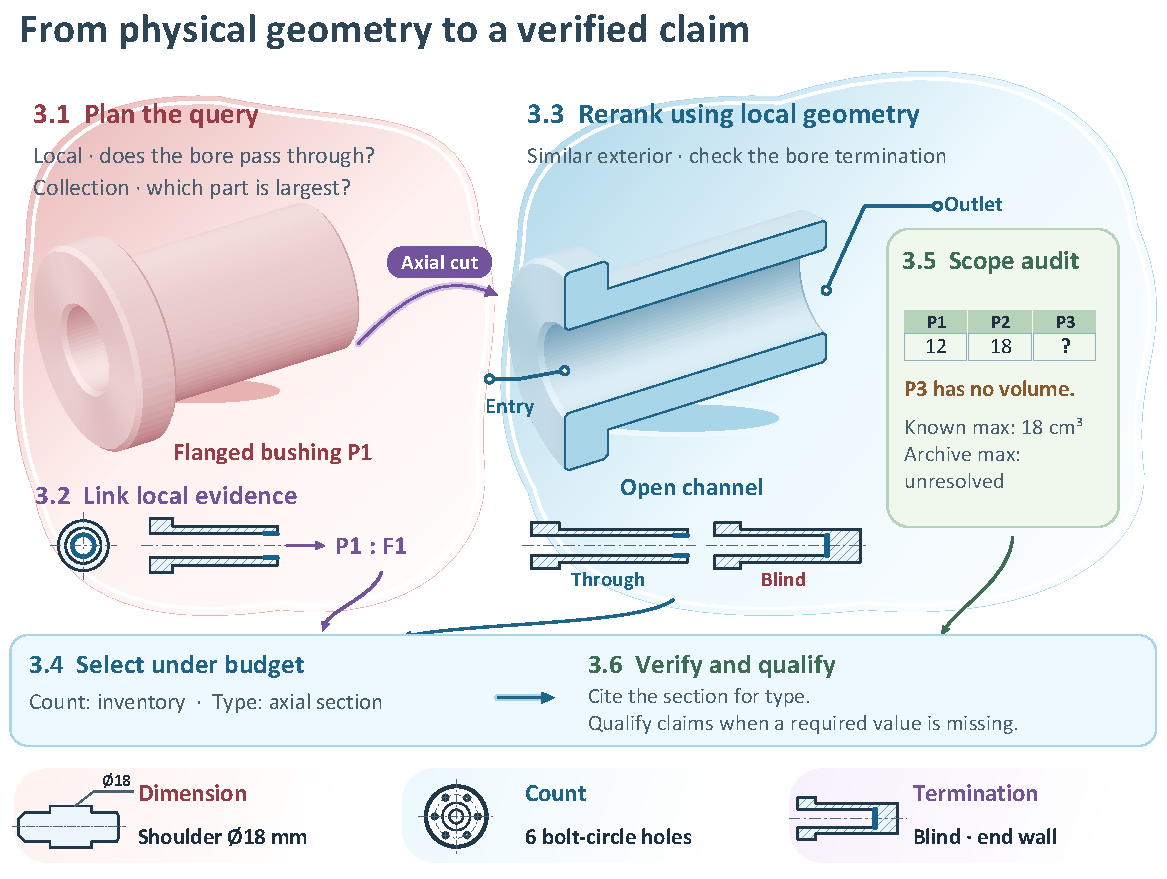
\includegraphics[width=\linewidth]{figures/study-plate.pdf}
\caption{The six method stages around a flanged bushing. The synthetic cutaway identifies the entry and outlet that support a local termination claim. The registry illustrates a different requirement: removing P3's volume in Step~3 of Figure~\ref{fig:geoevidence-comparison}B leaves the collection maximum unresolved. Both kinds of record enter budgeted selection and claim verification. The bottom examples illustrate dimension readout, feature counting, and termination judgment.}
\label{fig:method-map}
\end{figure}

\subsection{Problem definition}
\label{sec:problem}
Let $q$ be a question over an archive of drawing observations and, where available, native CAD attributes. We maintain an evidence index $\mathcal E$ and a registry $\mathcal P$ of part identifiers. The registry records the parts eligible under the declared scope, including parts whose attributes are missing. For a given part $p$, the index supplies the records
\begin{equation}
  \mathcal E_p=\{e\in\mathcal E:p(e)=p\}.
\end{equation}
A query plan specifies a nonempty set of conditions $C$, a scope, and an optional aggregate operator. A request for the largest part by volume, for example, specifies a property, a population, and a maximum operator:
\begin{equation}
  \operatorname{plan}(q)=(C,\operatorname{scope}(q),\operatorname{op}(q)).
\end{equation}
The reader receives a set $S$ drawn from a candidate pool $U$. The context budget $B$ bounds the sum of the positive record costs $b(e)$:
\begin{equation}
  S\subseteq U,\qquad b(S)=\sum_{e\in S}b(e)\le B .
  \label{eq:method-budget}
\end{equation}
Every engineering judgment $j$ carries its condition identifiers $C_j$ and its cited evidence identifiers $I_j$. The result is an answer with a claim-level audit trail:
\begin{equation}
  \operatorname{output}(q)=
  \bigl(\operatorname{answer},\,\{(j,C_j,I_j)\}_{j\in\operatorname{claims}}\bigr).
\end{equation}
Table~\ref{tab:method-notation} lists the notation shared across stages.

Consider two requests about the bushing in Figure~\ref{fig:method-map}. To determine whether its central bore passes through the part, the relevant observations concern one identified feature. A section through the bore axis can settle the question if it shows the channel meeting both exterior faces. To identify the bushing with the largest volume in an archive, every eligible part contributes a potential counterexample. Adding an omitted part can change the winner even if every previously read dimension was correct. This difference determines how $U$ is assembled before the budget in Eq.~\eqref{eq:method-budget} is applied.

The distinction between $U$ and $S$ also matters for a question with several clauses. Suppose the reader is asked for both a bore diameter and its termination. A diameter annotation supports a size claim, while a section establishes where the channel ends. Giving each judgment its own $C_j$ and $I_j$ makes it possible to identify a missing sectional observation even when the diameter has been read correctly. The budget controls what the reader sees. The population named in the question remains the same.

\begin{table}[!htbp]
\centering
\caption{Notation used across the method.}
\label{tab:method-notation}
\small\vspace{4pt}
\renewcommand{\arraystretch}{1.08}
\begin{tabular}{@{}l@{\hspace{1em}}p{.67\linewidth}@{}}
\hline
Symbol & Meaning \\ \hline
$q,\ C,\ c$ & Question, its verification conditions, and one condition.\\
$\mathcal P,\ p,\ f$ & Declared part registry, part identifier, and feature identifier within a part.\\
$\mathcal E,\ e$ & Evidence index and one citable record.\\
$F,\ R,\ A,\ L$ & CAD faces, view regions, attributed properties, and source locators of a record.\\
$K,\ U,\ S$ & Candidate depth, available evidence pool, and selected evidence.\\
$B,\ b(e)$ & Context budget and positive cost of record $e$.\\
$h(e,c),\ H_c(S)$ & Support for condition $c$ from one record and best support in $S$.\\
$w_c,\ \lambda$ & Condition weight and redundancy penalty.\\
$a,\ D_a$ & Requested attribute and parts with a usable value for it.\\
$j,\ C_j,\ I_j$ & Answer claim, attached conditions, and cited identifiers.\\
\hline
\end{tabular}
\end{table}

\FloatBarrier
\subsection{Construction of local geometric evidence units}
\label{sec:method-units}
Each property stays attached to the feature it describes. Each feature record carries a stable key $(p,f)$, face identifiers $F$, regions $R$, a property map $A$, and source locators $L$:
\begin{equation}
  e=(p,f,F,R,A,L),\qquad \operatorname{id}(e)=(p,f).
\end{equation}
The record also stores its type and cost. An empty $F$ is admissible for a drawing-only record. Each region identifies a view, an image and a normalized box. For a crop with page bounds $(x_0,y_0,x_1,y_1)$, a crop-relative point $(u,v)$ maps back to
\begin{equation}
  T(u,v)=\bigl(x_0+(x_1-x_0)u,\;y_0+(y_1-y_0)v\bigr).
\end{equation}
Applying $T$ to the two box corners recovers a location on the original page. Boxes from different projections may occupy unrelated coordinates. Their grouping instead uses the identity assigned to each input record $r$:
\begin{equation}
  G_{pf}=\{r:(p(r),f(r))=(p,f)\}.
\end{equation}
The coordinate transform can be audited independently of feature interpretation. Consider a crop spanning $(0.20,0.10)$ to $(0.60,0.50)$ on the page. A detection from $(0.25,0.25)$ to $(0.75,0.75)$ inside that crop maps to $(0.30,0.20)$ and $(0.50,0.40)$ on the sheet. Applying $T$ once allows the reader to revisit the source location even if the crop was resized for retrieval. Identifying the same physical bore in a different projection requires the separate correspondence key $(p,f)$.

\begin{figure}[!ht]
\centering
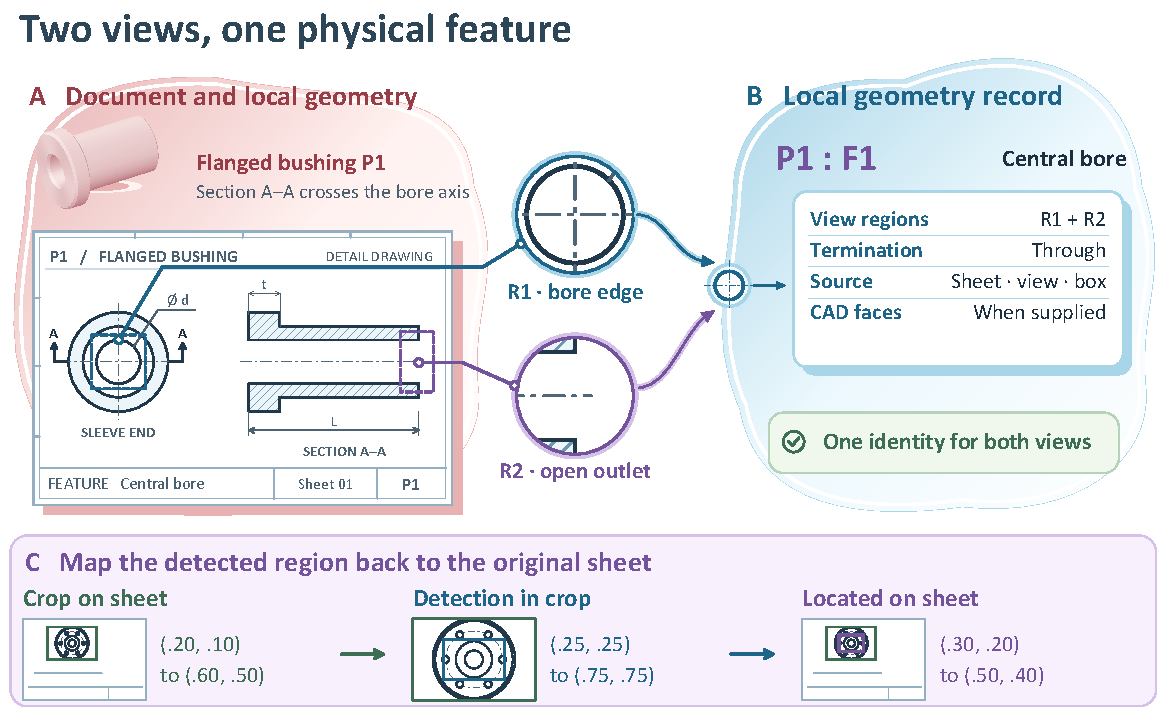
\includegraphics[width=\linewidth]{figures/feature-record-plate.pdf}
\caption{Construction of a local geometric evidence unit. (A) Detail windows enlarge the marked bore edge and outlet from the same source drawing. (B) The key P1:F1 retains both view locators and the observed termination. (C) A separate coordinate example follows a detection from a cropped view back to its original sheet. Each pair of coordinates specifies a corner of the normalized box.}
\label{fig:method-unit}
\end{figure}

Within a group, the merge pools the face, region, and source sets, retaining distinct view locators:
\begin{equation}
 (F,R,L)_{pf}=
 \left(\bigcup_{r\in G_{pf}}F_r,\ \bigcup_{r\in G_{pf}}R_r,\
       \bigcup_{r\in G_{pf}}L_r\right).
\end{equation}
Common keys in $A$ must agree. Categorical values require equality. Numeric values $u,v$ in the same units agree when
\begin{equation}
 |u-v|\le \max\{\epsilon,\epsilon\max(|u|,|v|)\}.
\end{equation}
The default merge tolerance is $\epsilon=10^{-6}$ in the stored units. Conflicting properties or identity metadata cause the merge to fail. Figure~\ref{fig:method-unit} shows how two projections retain distinct roles after consolidation. Assigning the shared key requires a source correspondence. Similar contours alone leave the identity unresolved.

The bushing illustrates the ambiguity. Several circles share a center in the sleeve-end view, yet their boundaries belong to the bore, the sleeve exterior, or the flange. Attaching the bore diameter to the flange edge would preserve a plausible numeric value under the wrong owner. Keeping the individual locators after consolidation lets an inspector follow a dimension back to its referenced edge and a termination judgment back to its sectional contour. The merge tolerance $\epsilon$ governs agreement between stored values. A manufacturing tolerance attached to a dimension is a separate engineering property with its own source.

\subsection{Global candidate search and modeling of local geometric differences}
\label{sec:method-rank}
For a visual query profile, let $z_q$ and $z_p$ denote the reference and candidate part embeddings from a frozen CLIP encoder~\cite{radford2021clip}. The first stage retrieves the $K$ highest cosine scores:
\begin{equation}
 g_p=\frac{z_q^\top z_p}{\|z_q\|\,\|z_p\|},\qquad
 P_K=\operatorname{TopK}_{p\in\mathcal P}\,g_p .
\end{equation}
Zero-norm vectors receive score zero. Text-only queries can supply candidate identifiers directly. Pairwise geometric reranking requires a reference profile and candidate profiles.

For each query feature $f$ with embedded regions, compare its crops with candidate crops of the same feature type. With $z_r$ the embedding of region $r$ and $R_p$ the candidate's embedded regions, the best available alignment is
\begin{equation}
 d_f(p)=\max_{\substack{r\in R_f,\ t\in R_p\\
                   \operatorname{type}(t)=\operatorname{type}(f)}}
                   \cos(z_r,z_t).
\end{equation}
Let $M$ contain features with a matched score above $-1$, and let $n$ count query features with embedded regions. Three statistics summarize the strength and extent of alignment:
\begin{equation}
 d_{\max}=\max_{f\in M}d_f,\qquad
 \bar d=\frac{1}{|M|}\sum_{f\in M}d_f,\qquad
 \rho_f=\frac{|M|}{n}.
\end{equation}
For critical attribute $a$, let $A_p[a]$ denote the set of its observed values across the part. On the keys $J$ observed for both profiles, the agreement and disagreement fractions are
\begin{equation}
 m_+=\frac{\sum_{a\in J}\mathbf1\{A_q[a]=A_p[a]\}}{|J|},\qquad
 m_-=\frac{\sum_{a\in J}\mathbf1\{A_q[a]\ne A_p[a]\}}{|J|}.
\end{equation}
Empty pools and zero denominators in these summaries return zero. If $v_q,v_p$ count distinct views, $\rho_v=\min(1,v_p/\max(1,v_q))$ measures view availability. The learned score uses seven inputs:
\begin{equation}
 x_p=(g_p,d_{\max},\bar d,m_+,m_-,\rho_f,\rho_v),\qquad
 s_p=\sigma\!\left(\operatorname{MLP}_{\theta}(x_p)\right).
\end{equation}
The MLP has two ReLU hidden layers of widths 16 and 8. A fixed weighted scorer over $x_p$ is available when a trained checkpoint is absent. Candidate parts are ordered by the chosen score before their evidence is collected.

Two bushings can have nearly identical $g_p$ because their outer envelopes and front openings match. Their strongest crop scores $d_{\max}$ may also be close when the best pair depicts only the opening. Suppose hole count and bore type are the only comparable attributes. For a through-bore reference, a blind-bore candidate with the correct count gives $(m_+,m_-)=(0.5,0.5)$, while a candidate matching both properties gives $(1,0)$. The scorer can use this distinction even when the global descriptor changes little. If bore type is missing, it drops out of $J$ and agreement on count alone can again give $m_+=1$. A high score in that case warrants inspection of a sectional record before making a claim about termination.

Training pairs are mined among visual neighbors. A weak label compares their full critical-attribute signatures $\operatorname{sig}$ when at least one critical value is observed across the pair:
\begin{equation}
 y_{qp}=\mathbf1\{\operatorname{sig}(q)=\operatorname{sig}(p)\}.
\end{equation}
A change from a blind bore to a through bore can yield a negative pair at high $g_p$. Unequal annotation completeness can also yield $y_{qp}=0$. For an editable CAD variant, a controlled pair requires regenerating the affected views and descriptors after the edit. Binary cross-entropy trains the reranker:
\begin{equation}
 \mathcal L(\theta)=-\operatorname{mean}_{(q,p)}
 \big[y_{qp}\log s_p+(1-y_{qp})\log(1-s_p)\big].
\end{equation}
Here $\sigma$ is the logistic function. Only $\theta$ is optimized. An original part, its variants and their projections inherit one family identifier. Writing $\mathcal F$ for sets of families, the split enforces
\begin{equation}
 \mathcal F_{\rm train}\cap\mathcal F_{\rm test}=\varnothing .
\end{equation}
A pair enters a partition only when both endpoints belong to it. Pairs crossing the boundary are discarded.

The matching rule explains why feature identity is still needed downstream. Two query features can attain their largest crop similarities against the same candidate region, since the maxima in $d_f(p)$ are computed independently. Thus $\rho_f$ measures the availability of plausible matches and cannot establish a one-to-one correspondence for counting. Similarly, renderings of one edited part can produce many nearly identical test pairs. Holding out the entire family makes ranking evaluation sensitive to transfer across parts. First-stage recall sets a further limit on this evaluation because a reranker can reorder only the parts present in $P_K$.


\subsection{Question decomposition and complementary evidence selection under a budget}
\label{sec:method-selection}
A rule-based parser matches property aliases in $q$ and identifies an operator such as maximum, minimum, ordering, or distinct count. A named property normally gives one condition. If none is recognized, the normalized question becomes a descriptive condition. Each condition carries its requested keys, priority, and an exhaustive-scope flag:
\begin{equation}
 c=(\operatorname{keys}(c),w_c,\operatorname{scope}(c),
             \operatorname{exhaustive}(c)).
\end{equation}
Figure~\ref{fig:method-budget} illustrates the marginal gain for two requested properties.

\begin{figure}[!ht]
\centering
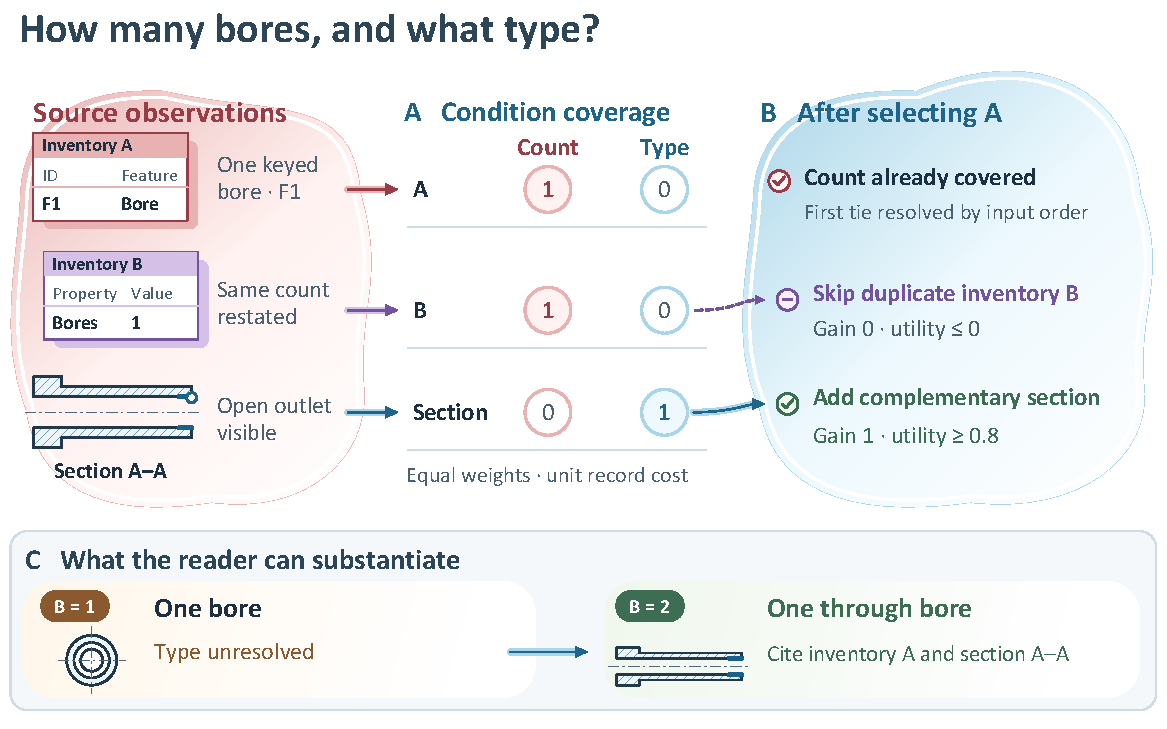
\includegraphics[width=\linewidth]{figures/selection-plate.pdf}
\caption{Complementary evidence selection for an illustrative part with one bore. The source excerpts show two inventories and an axial section. (A) The inventories cover the same count condition. (B) Input order breaks the initial tie. With unit costs, equal weights, and $\lambda=0.2$, adding the section after inventory A has utility at least $0.8$. (C) A one-record answer leaves termination open. At two records, the reader can cite both count and type.}
\label{fig:method-budget}
\end{figure}

For a local condition, $h(e,c)$ measures how much relevant information a record exposes. Write $J_c=\operatorname{keys}(c)$ and let $T_c,T_e$ be the token sets of the description and of the record summary plus feature type. The default support score is
\begin{equation}
 h(e,c)=
 \begin{cases}
 |J_c\cap\operatorname{keys}(A_e)|/|J_c|,&J_c\ne\varnothing,\\
 |T_c\cap T_e|/\max(1,|T_c|),&J_c=\varnothing .
 \end{cases}
\end{equation}
Property presence indicates that an observation can be inspected. Its value still determines the engineering answer. For an exhaustive condition, only a structured aggregate for the requested attribute receives credit:
\begin{equation}
 h(e,c)=
 \begin{cases}
 1,&\text{matching aggregate with complete scope},\\
 0.4,&\text{matching aggregate with incomplete scope},\\
 0,&\text{otherwise}.
 \end{cases}
 \label{eq:aggregate-support}
\end{equation}
The partial score lets a bounded context carry an explicit warning. Each condition retains the strongest selected support, initialized at zero:
\begin{equation}
 H_c(S)=\max\bigl(\{0\}\cup\{h(e,c):e\in S\}\bigr).
\end{equation}
Writing $[u]_+=\max(0,u)$, the additional weighted coverage offered by a candidate is
\begin{equation}
 \Delta(e\mid S)=\sum_{c\in C}w_c\,[h(e,c)-H_c(S)]_+ .
\end{equation}
A request for both hole count and bore type illustrates the choice of decomposition. With separate conditions $c_1$ and $c_2$, an inventory can fully support $c_1$ and a section can fully support $c_2$. If both keys were bundled into one condition, each record would score $1/2$ and their maximum would remain $1/2$ after both were selected. The maximum in $H_c(S)$ therefore favors conditions that can each be verified from one record. Properties that must hold for the same bore still require an identity check. Two units from different parts may cover both property names without answering the joint question about P1.

Redundancy uses Jaccard overlap $J(X,Y)=|X\cap Y|/|X\cup Y|$, with zero for an empty union. For distinct records $e,t$, let $i_p$ indicate a shared part and $i_t$ a shared feature type. With $T'_e$ denoting summary tokens, define
\begin{equation}
 r(e,t)=\max\{i_p J(F_e,F_t),\,J(T'_e,T'_t),\,0.5\,i_p i_t\}.
\end{equation}
Identical identifiers give $r(e,t)=1$. With a default $\lambda=0.2$, the priority of a feasible record is its net marginal gain per unit cost:
\begin{equation}
 u(e\mid S)=
 \frac{\Delta(e\mid S)-\lambda\max_{t\in S}r(e,t)}{b(e)} .
\end{equation}
The redundancy term is zero for $S=\varnothing$. Starting from that set, the selector takes the highest positive priority that fits:
\begin{equation}
 e^* \in \underset{\substack{e\in U\setminus S\\b(S)+b(e)\le B}}{\arg\max}\ u(e\mid S),
 \qquad S\leftarrow S\cup\{e^*\}\quad\text{if }u(e^*\mid S)>0 .
\end{equation}
Selection stops when all $H_c(S)=1$, the feasible set is empty, or its best gain is nonpositive. The reported coverage is the unweighted mean of $H_c(S)$.

In Figure~\ref{fig:method-budget}, taking inventory A changes the coverage vector from $(0,0)$ to $(1,0)$. Inventory B then has $\Delta=0$ even if its wording closely matches the question. For the sectional record, $\Delta=1$ and $b(e)=1$, so with $\lambda=0.2$ its utility is at least $0.8$ for any admissible redundancy score. At $B=2$ the section fits and the final vector is $(1,1)$. Reducing the budget to $B=1$ leaves bore type unresolved. Reporting the uncovered condition identifies the observation lost to the budget. Equal priorities can make the choice order-dependent, and greedy selection need not yield the globally best subset.



\subsection{Global candidate-set completeness and missing-attribute checks}
\label{sec:method-scope}
A global maximum is a statement about $\mathcal P$. Even perfect ranking within $P_K$ gives no account of an omitted part. For a recognized operator with a single attribute $a$, the structured path scans the registry independently of $K$. Assume consistent units and attribute semantics at ingestion. Define the observed and missing populations by
\begin{equation}
 D_a=\{p\in\mathcal P:\text{a usable value }a(p)\text{ is recorded}\},
 \qquad M_a=\mathcal P\setminus D_a .
\end{equation}
For numerical comparisons, a usable value must be numeric and applicable to the specified part. Repeated consistent values produce one row per part. Incompatible values raise a conflict. Let $d=1$ signify that the registry was declared complete for this scope. The completeness flag is
\begin{equation}
 \operatorname{complete}(a)=
 \mathbf1\{d=1,\ |\mathcal P|>0,\ M_a=\varnothing\}.
 \label{eq:method-complete}
\end{equation}
The registry flag and the missing set test independent assumptions. An index built solely from records containing a volume would make $M_a$ empty by construction. A separately declared list of eligible parts allows a drawing with no volume entry to remain visible during the scan. Conversely, all known parts may have values while the archive itself is only a sample. In that case $d=0$ prevents promotion of a sample maximum to a collection-wide claim.

Usability also depends on the meaning of $a$. Part volume and bounding-box volume may both be expressed in cubic millimetres, but changing an internal bore can alter one while leaving the other unchanged. The index therefore distinguishes their property keys. Comparable units are an ingestion requirement for numeric comparisons. A value whose units have not been resolved cannot justify an exact physical comparison merely because it can be parsed as a number.

The scan preserves the part identifier, value, and source evidence identifier in each row. For a maximum with $D_a\ne\varnothing$, its value and tied winners are
\begin{equation}
 v^*=\max_{p\in D_a}a(p),\qquad
 W=\{p\in D_a:a(p)\simeq v^*\},
\end{equation}
where $\simeq$ uses numerical comparison tolerance. Minima reverse the comparison. Ordering retains the per-part rows, and a distinct count groups equal attribute values. The result is packaged as one citable record $e_a$ with provenance and a completeness flag. The reader's candidate pool becomes
\begin{equation}
 U=\left(\bigcup_{p\in P_{\rm kept}}\mathcal E_p\right)\cup\{e_a\},
\end{equation}
where $P_{\rm kept}$ is the retained shortlist. For a local request the last term is omitted. The scan is exhaustive over the declared registry, but its result still competes for context budget. If $n_{\rm out}$ counts ties, ordered rows, or distinct groups according to the operation, its cost is
\begin{equation}
 b(e_a)=\max(1,n_{\rm out}/10).
\end{equation}
For the volumes in Step~3 of Figure~\ref{fig:geoevidence-comparison}B, $D_a=\{\mathrm{P1},\mathrm{P2},\mathrm{P3}\}$ gives $v^*=24\,\mathrm{cm}^3$. Removing P3's value leaves $M_a=\{\mathrm{P3}\}$. The largest observed volume is then $18\,\mathrm{cm}^3$ and the collection maximum remains unresolved.

The scan and the context budget constrain different operations. The store can inspect all eligible rows while the reader receives an aggregate with the winning identifiers and the observed and expected counts. A tie increases the number of output items, and a long ordering may cost more than $B$. If the aggregate cannot enter $S$, the reader lacks a citable basis for an exhaustive answer even when the scan is complete. Inspecting both $\operatorname{complete}(a)$ and $I(S)$ distinguishes this case from an actual gap in the archive.

\subsection{Answer consistency checks and uncertainty handling}
\label{sec:method-verification}
The reader receives $q$, the conditions, selected records, and the coverage report. The citation vocabulary is generated directly from the supplied context:
\begin{equation}
 I(S)=\{\operatorname{id}(e):e\in S\}.
\end{equation}
Identifiers inside an aggregate trace locate contributing rows. The reader cites the selected aggregate itself.

For example, a maximum-volume record can name P3 and retain the identifier of the row that supplied its volume. Citing only P3's row would show that P3 has that value. The aggregate also records the population over which P3 was compared, which is needed for the word \emph{largest}. The nested identifier remains available to trace the measurement, while the claim-level citation points to the record that supports the comparison.

For claim $j$, sources outside the available context are detected by
\begin{equation}
 \operatorname{unknown}(j)=I_j\setminus I(S).
\end{equation}
For condition $c$ named by the claim, at least one cited record must reach the threshold $\tau_c$. Writing $I_j^+(c)$ for eligible citations gives
\begin{equation}
 I_j^+(c)=\{\operatorname{id}(e)\in I_j:e\in S,\ h(e,c)\ge\tau_c\},
 \qquad
 \tau_c=\begin{cases}1&\text{exhaustive},\\10^{-12}&\text{local}.\end{cases}
\end{equation}
The local threshold checks that a citation has positive support. A partial aggregate falls below the exhaustive threshold by Eq.~\eqref{eq:aggregate-support}. Each accepted claim must cite known records and attach them to known conditions:
\begin{equation}
 \begin{aligned}
 \operatorname{ok}(j)={}&
 \mathbf1\{\varnothing\ne I_j\subseteq I(S),\
             \varnothing\ne C_j\subseteq C,\\[-2pt]
 &\hspace{30mm} I_j^+(c)\ne\varnothing\ \text{for every }c\in C_j\}.
 \end{aligned}
\end{equation}
Finally, the claims must jointly address the requested conditions. With $\mathcal J$ the submitted claims, the acceptance rule is
\begin{equation}
 \operatorname{valid}=
 \mathbf1\!\left\{\ \bigcup_{j\in\mathcal J} C_j=C,\
                   \operatorname{ok}(j)=1\ \text{for all }j\in\mathcal J\right\}.
\end{equation}
A failed check identifies the unsupported claims, unknown citations, or uncovered conditions. If a volume is missing, the prompt directs the reader to qualify the scope. If the required sectional observation is absent, bore termination remains unresolved.

These checks separate an incomplete answer from an unsupported one. An answer reporting only a diameter can cite a valid dimension yet leave the requested bore type uncovered. An answer reporting both properties with an invented section identifier fails the citation check. A third failure can pass the structural checks when a reader cites a real record containing bore type but reverses \emph{blind} and \emph{through} in its prose. Checking $I_j^+(c)$ alone cannot detect that reversal. The attribute value and source locator make it possible to audit the discrepancy against the drawing. Accordingly, coverage measures which conditions are represented, and the validity flag tests the claim-to-record links. Neither is a calibrated probability that the engineering answer is correct.


\clearpage
\section{Experiments}
\label{sec:experiments}

\begin{table}[!ht]
  \centering
  \caption{Preliminary CAD question answering results (\%).}
  \label{tab:retrieval-comparison}
  \footnotesize
  \setlength{\tabcolsep}{1.6pt}
  \renewcommand{\arraystretch}{1.15}
  \resizebox{\linewidth}{!}{%
  \begin{tabular}{@{}l*{4}{@{\hspace{4pt}}ccc}@{}}
    \toprule
    & \multicolumn{3}{c}{DeepCAD} & \multicolumn{3}{c}{TriView2CAD}
    & \multicolumn{3}{c}{FCM} & \multicolumn{3}{c}{CADVQA} \\
    \cmidrule(lr){2-4}\cmidrule(lr){5-7}\cmidrule(lr){8-10}\cmidrule(lr){11-13}
    Method & Acc & Recall & F1 & Acc & Recall & F1
           & Acc & Recall & F1 & Acc & Recall & F1 \\
    \midrule
    No retrieval & 88.00 & 93.00 & 93.00 & 81.00 & 93.67 & 93.67
                 & 0.00 & 33.16 & 41.27 & & & \\
    \midrule
    \multicolumn{13}{@{}l}{\itshape Text-based retrieval} \\
    \inputtablerows text-full-rows.tex
    \midrule
    \multicolumn{13}{@{}l}{\itshape Pixel-based retrieval} \\
    PixelRAG (base) & 75.00 & 85.50 & 85.50 & 85.00 & 95.00 & 95.00
                    & 0.00 & 38.78 & 47.50 & & & \\
    PixelRAG & 78.00 & 87.00 & 87.00 & 86.00 & 95.33 & 95.33
             & 0.00 & 39.29 & 46.53 & & & \\
    \midrule
    \multicolumn{13}{@{}l}{\itshape Fix-based retrieval} \\
    GeoEvidence-RAG (ours) & & & & & & & & & & & & \\
    \bottomrule
  \end{tabular}}
  \par\smallskip
  \parbox{\linewidth}{\raggedright
    Rows marked $\dagger$ use local Qwen3-VL-2B-Instruct (Q4\_K\_M).
    The other populated rows use DeepSeek Flash. All methods receive the target image.
    The text baselines share OCR regions and keep up to two passages ranked by BM25~\cite{robertson2009bm25}
    or by cosine similarity of BGE-M3 dense embeddings~\cite{chen2024m3}.
    Pixel retrieval adds the two highest-scoring tiles from four overlapping crops
    of the target image. PixelRAG (base) uses Qwen3-VL-Embedding-2B and
    PixelRAG applies the published LoRA checkpoint.
    The DeepSeek rows use 100 derived DeepCAD sketches and 100 TriView2CAD drawings.
    The full local runs use one derived sketch per official DeepCAD test model
    and all 200,000 public TriView2CAD synthetic drawings.
    FCM uses all 53 labeled subtractive-manufacturing images. Their OCR yielded no
    passages above the confidence threshold, so the text systems used direct visual answers.
    Acc is exact match per sample. Recall and F1 are micro-averaged over answer items.
    Blank cells are pending evaluation.}
\end{table}
\FloatBarrier

\begingroup
\interlinepenalty=10000
\bibliographystyle{elsarticle-num}
\bibliography{references}
\endgroup
\end{document}
